\section{Train Path Planning and Train Path Assignment}
\label{chap:methods}
%
In this section we briefly describe our modelling approach to automatically create timetables. It is divided into two main parts: First, we precalculate slots, which are located on the most frequently used part of the infrastructure (Section~\ref{chap:Konstruktion}). Therefore, we extend the idea of \cite{O:2009}. The second part is the train path assignment (Section~\ref{chap:Belegung}), based on the idea of \cite{N:1998, N:2015} and \cite{NO:2014}, where some single train paths are assigned to a complete timetable.


\subsection{Train Path Calculation}
\label{chap:Konstruktion}
%
This section will give a brief overview of the process used for creating a train path. The entire process consists of three main steps. First, we search one or more different routes through the infrastructure. In the second step we create a network of discrete building blocks (called snippets) along these routes for which we calculate travel and blocking times. Finally, we put these snippets together to form a non conflicting train path. The same process is used to calculate train paths for individual requests as well as the precalculated slots for the annual timetable. For the slots we consider frequently travelled relations, each starting and ending in one Betriebstelle. For each relation we consider up to three different train characteristics, chosen to be representative for most of the traffic expected on the relation.


\subsubsection{Routing}
To reduce the problem size, our first step consists of finding routes that could be relevant for the train. We use an A* algorithm for finding a shortest route on our infrastructure, which is a digital representation of the German railyway network and it containing all necessary information like maximal allowed mass, width or length. The algorithm utilizes geo coordinates for calculating the beeline distance as the lower bound. The infrastructure of Deutsche Bahn is divided into sections called \emph{Betriebstellen}.
For each Betriebstelle we keep a list of all possible ways to traverse it. Each possibility is termed a \emph{Fahrweg}. The Fahrwege form a graph where each Fahrweg is a vertex, with directed edges indicating which Fahrweg is a direct successor of another. The edge costs are based on the Fahrwege lengths.
But as certain Fahrwege are preferred to others we multiply the cost with factor which is closer to one for more desirable Fahrwege. This way the use of intersections and the use of tracks from the opposite direction can be discouraged. It is this graph we use for finding routes for our train paths.

While exploring the graph the algorithm filters out all paths, which are incompatible with the characteristics of the train.
As it is not always the best option to use the shortest path, we create multiple alternative routes. For searching the subsequent routes, we increase the costs of edges that where used in already found routes. A route is only accepted as a real alternative if it differs from all already calculated ones in at least one Betriebstelle. We set an upper limit to the length of alternative routes which is a multiple ($1.3$ in the experiments) of the shortest route found.


\subsubsection{Snippet Creation}
%
For each route we calculate the travel and blocking times that would be required for a train using the route without intermediate stops. To enable stopping, we search for all tracks that could be used for a stop of the train along the route. A track is only considered for stopping, if it branches off the main route and joins it again within a single Betriebstelle. For each such track we create one snippet leading from the main route to the stop and one from the stop to the main route. These snippets have a length of $7$km, a length that ensures that acceleration and deceleration to and from the main travel speed is always possible within the snippet. For each snippet we again calculate travel and blocking times. In order to connect these snippets with the main route, we cut it into snippets at the points where our stopping snippets branch off it or join it back. In addition to these stop snippets, we create snippets for alternative non stopping traversals of a Betriebstelle for all tracks that traverse the Betriebstelle similar to the original main route. Sometimes it can be beneficial for a train to travel with less than its maximum speed to match the speed of a preceeding train without stopping unnecessarily. To enable this we create alternatives of each snippet with reduced maximum speeds.

This way we get a directed, acyclic graph of snippets representing the possible ways the train can travel along each route including intermediate stops. Each snippet has travel and blocking times calculated. A path from a source snippet (those without predecessors) to a sink snippet (without successors) will always represent a valid train path (without a specific starting time of the train).


\subsubsection{Train Path Calculation}
%
The last step to calculate the train path is to determine a starting time and a path through the snippet graph such that no blocking time is in conflict with another train path and the number of stops is minimized. For each snippet we can calculate the possible departure times of the snippet that are not conflicting with other trains by projecting the blocking times of other trains back to the snippets start. This way we get a list of intervals for each snippet where each interval represents the allowed start times. Next we reduce the intervals further to ensure that only such intervals remain that can be reached by one of the snippets predecessors. For each snippets we calculate the possible arrival times given the known departure intervals. Note that for a snippet not ending in a stop, the resulting intervals will have the same length but are shifted by the travel time of the snippet. For stopping snippets the intervals can increase in size as long as the stop is not used by a different train. For each snippet we take the union of all its predecessors arrival intervals and intersect them with the possible departures of the snippet. This yields the new departure times of the snippet. As the snippet graph is directed and acyclic, we can find a topological ordering of the snippets such that this reduction of departure times needs to be done only once per snippet.

The possible arrival times of the sink snippets will now be such that there must exist a non conflicting valid train path arriving at the given time. We calculate train paths by choosing the earliest arrival time. For a given arrival time we can select the predecessor snippets that have a compatible departure time. From those we select those that lead to the least number of stops (we prefer non stopping predecessors) first and then to the latest departure. The resulting train path is guaranteed to be conflict free, while keeping the number of stops and travel time low. The algorithm runs sufficiently fast, requiring $\mathcal{O}(m+n)$ calculations where $m$ is the number of snippets and $n$ is the number of edges in the snippet graph.

%
\begin{figure}[tb]
	\centering
	% If you include a JPG file,
	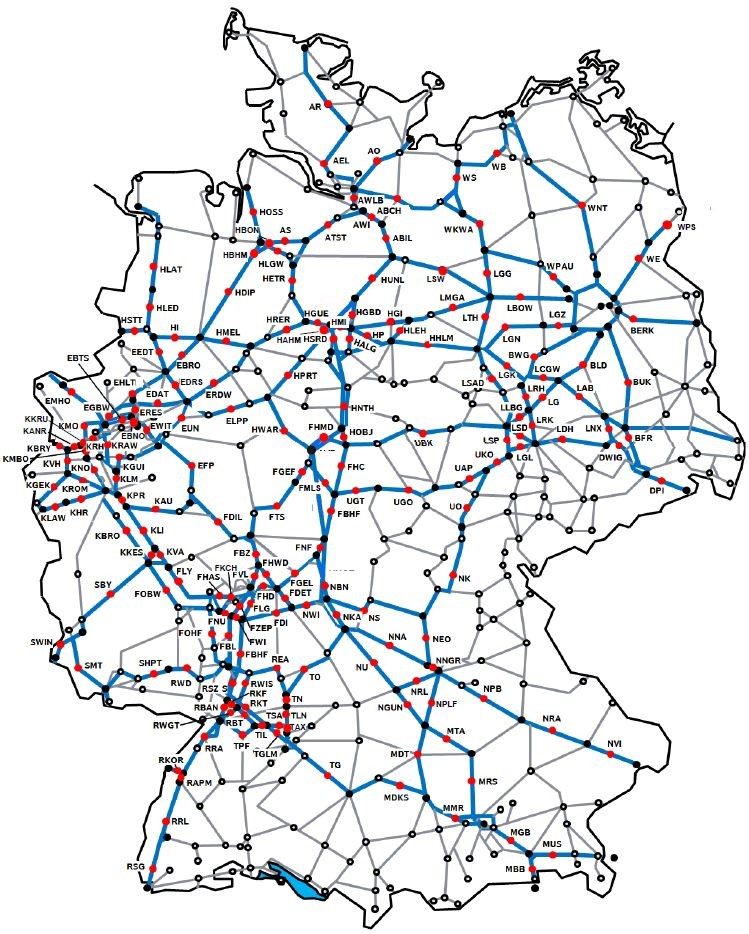
\includegraphics[scale=0.40]{Bilder/STA-Karte.jpg}
	% Else if you include an EPS file
	%    (it may need an interpreter for the PostScript language, e.g. Ghostscript),
	%\includegraphics[scale=0.30]{Fig1_Track.eps}
	\caption{A macroscopic map of the infrastructure administrated by DB Netze. The created slots are indicated by blue lines. The time dependency is neglected for a better overview.}
	\label{fig:STAKarte}
\end{figure}


\subsection{Train Path Assignment}
\label{chap:Belegung}
%
As a result of the slot calculation presented in the previous section (Section~\ref{chap:Konstruktion}), we are provided with a set of slots starting and ending at a specific Fahrweg at a specific time. So, the slots form a graph, we call \G\, for later reference, where the slots are the edges and the tuple of Fahrweg and point in time are the vertices. In a process consisting of four steps, this graph is used to assign train paths to the requests made by customers. First, we map the requests of the customer to the graph \G, resulting in so-called \emph{break-in} and \emph{break-out points}. Then, we search for the shortest path within \G\, using slots. In the third part, we calculate train paths from the start of a request to the break-in point and from the break-out point to the target of the request. Finally, we optimize the result for all requests using a column generation approach.

\subsubsection{Calculation of Break-in and Break-out Points}
%
As most customer requests do not start or end at vertices of the graph \G\, (compare Figure~\ref{fig:E-A-Pkte}), we need to map the start and end of a request to vertices of \G, which we call break-in and break-out points, respectively. Therefore, we calculate a number of different routes (10 in the experiment), using the A* algorithm previously described. Then, beginning at the start of the route, we consecutively check for each Fahrweg of each route whether it is associated to a vertex of the graph \G. If so, we found a break-in point and stop; otherwise no sequence of predefined slots can be used and the request has to be calculated individually. In order to find the break-out points, we repeat the above process starting from the end of each route.
%
\begin{figure}[tb]
	\centering
	% If you include a JPG file,
%	\includegraphics[scale=0.40]{EAPkte.jpg}
	% Else if you include an EPS file
	%    (it may need an interpreter for the PostScript language, e.g. Ghostscript),
	%\includegraphics[scale=0.30]{Fig1_Track.eps}
	\caption{A small section of Figure~\ref{fig:STAKarte}. The customer request starts at point $s$ and ends in $t$. The break-in and break-out points are marked as $\Box$ and $\Diamond$, respectively. The time dependency is neglected for a better overview.}
	\label{fig:E-A-Pkte}
\end{figure}

\subsubsection{Routing on Slots}
The mapping of a request previously described may not be unique (as indicated in Figure~\ref{fig:E-A-Pkte}), so that multiple sources and sinks have to be considered. Furthermore, due to the technical properties of the requests such as e.g.\ length, acceleration or width, the use of slots is restricted depending on the request. Those as well as the slots also have time restrictions. Thus we end up with a restricted, time-dependent multi-source-multi-sink shortest path problem to be solved for each request.

We use standard techniques to reduce the complexity of the problem like time expansion to tackle the time dependency. We model the multi-source-multi-sink problem with dummy edges from a super source and to a super sink. We cope with the restriction due to the technical properties by using dynamic filters. In that way, we are able to reduce the problem to a standard shortest path problem, which we solve using a Dijkstra algorithm.

\subsubsection{Individual Train Path Calculation}
In teh previous stps for each request, we either create a path of slots from a break-in point to a break-out point or we know that there isn't one. So in order to provide a train path from start to end for each request, we individually create train paths for the missing parts of each request, i.e.\ either both a train path from start to break-in point and a train path from break-out point to end or a train path from start to end. For those train path we use the approach presented in Section~\ref{chap:Konstruktion}. Consequently, after that step we provide exactly one train path per request.

\subsubsection{Optimization}
The process described above is sufficient if only one request hast to be fulfilled at a time like in the use case of the app. But if there is more than one request - like in the use case of annual timetable - the simple assignment of the shortest path for each request leads to conflicts between the train paths. We solve these conflicts using a column generation approach, where in each iteration we generate new train paths which resolve more conflicts than in the iteration before. Our experiments show, that the process terminates within up to 10 hours for sufficiently large problems (compare Section~\ref{chap:Netzfahrplan}).